\documentclass[]{article}
\usepackage{ctex}
\usepackage{geometry}
\usepackage{graphicx}
\usepackage{geometry}    %导入宏包
\geometry{a4paper,left=2.5cm,right=2.5cm,top=2cm,bottom=2.5cm}

\usepackage{fancyhdr}
\pagestyle{fancy}
\setlength\headheight{23pt}
\lhead{姓名: 罗啸\\ 学号: 2420173095}
\rhead{Page: \thepage\\ \today}
\chead{} \lfoot{} \cfoot{} \rfoot{}

%opening
\title{对傅里叶级数的理解}
\author{电子173班\quad 罗啸}

\begin{document}

\maketitle
\zihao {-4}
傅里叶级数是把任意周期函数或周期信号分解成一个(可能由无穷个元素组成的)简单振荡函数的集合,即正弦函数和余弦函数.

这里,我通过利用仿真软件进行实验的方法加深了对傅里叶级数的理解
\subsection*{一、方案设计}
由于任何满足迪利克雷条件的信号都能展开为傅里叶级数,为研究原始信号的输出波形和傅里叶展开后波形的关系,这里需设计一个原始电路和多电源叠加电路。为了方便后续的观察,原始电路采用周期明显的方波信号作为输入源,幅值设为1V,周期为20ms.设计电路图如图1所示,其中电阻阻值为1k.
\begin{figure}[htbp]
	\centering
	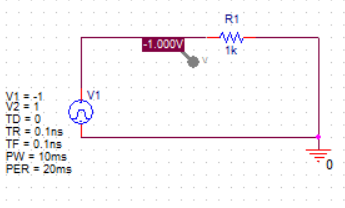
\includegraphics[height=3.0cm,width=3.5cm]{pics/0.png}%figures文件夹下的DSC.png图片,
	\caption{原始电路图}
\end{figure}

对于多电源叠加电路,采用计算的方法求出各阶电路的频率与幅值,再根据计算结果连接电路。

\subsection*{二、方波傅里叶级数展开}
对于方波信号,设其周期为$T$,幅值为1.则根据傅里叶级数的展开公式,可对其展开式进行求解.
$$a_{0}=\frac{1}{T}\int_{\frac{T}{2}}^{\frac{-T}{2}}x(t)dt=0$$
$$a_{n}=\frac{1}{T}\int_{\frac{T}{2}}^{\frac{-T}{2}}x(t)\cos{(n\omega_0t)}dt=0$$
$$b_{n}=\frac{1}{T}\int_{\frac{T}{2}}^{\frac{-T}{2}}x(t)\sin{(n\omega_0t)}dt$$

继续求解,得到:
$$b_{n}=\frac{4}{n\pi},n=1,3,5$$
$$b_{n}=0,n=2,4,6$$
根据傅里叶级数:$$f(t)=\frac{a_{0}}{2}+\sum_{n=1}^{\infty}{(a_{n}\cos{(2\omega_{1}t)}+b_{n}\sin{(2\omega_{1}t)})}$$

代入$a_n、b_n$将方波信号的傅里叶级数表示为:
$$f(t)=\frac{4}{\pi}\sum_{n=1}^{\infty}{\frac{1}{2n-1}\sin{(2n-1)\omega_0t}}$$

\subsection*{三、orCAD软件仿真}
利用orCAD软件对图1原始电路图进行仿真,得到输出波形见图2,该仿真波形为矩形脉冲源的输出信号,其幅值为1V,周期为20ms.
\begin{figure}[htbp]
	\centering
	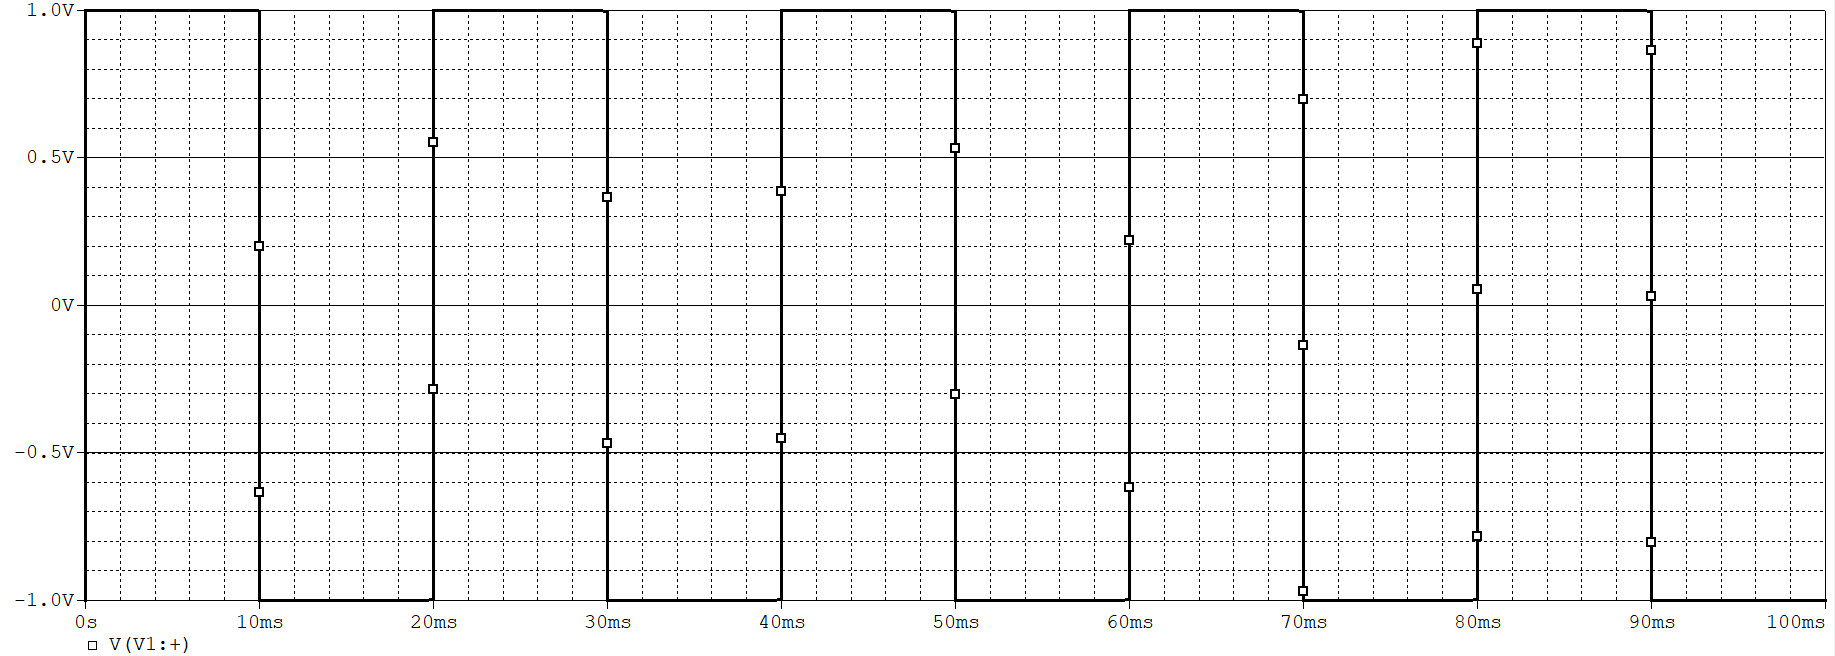
\includegraphics[height=4.0cm,width=12cm]{pics/01.png}%figures文件夹下的DSC.png图片,
	\caption{原始电路仿真图}
\end{figure}

\subsubsection*{3.1 三阶展开仿真}
对傅里叶级数进行三阶展开
$$f(t)=\frac{4}{\pi}{(\sin{(\omega_0t)}+\frac{1}{3}\sin{(3\omega_0t)}+\frac{1}{5}\sin{(5\omega_0t)})}$$

设计电路见图3,即采用三个正弦波电源叠加.
\begin{figure}[htbp]
	\centering
	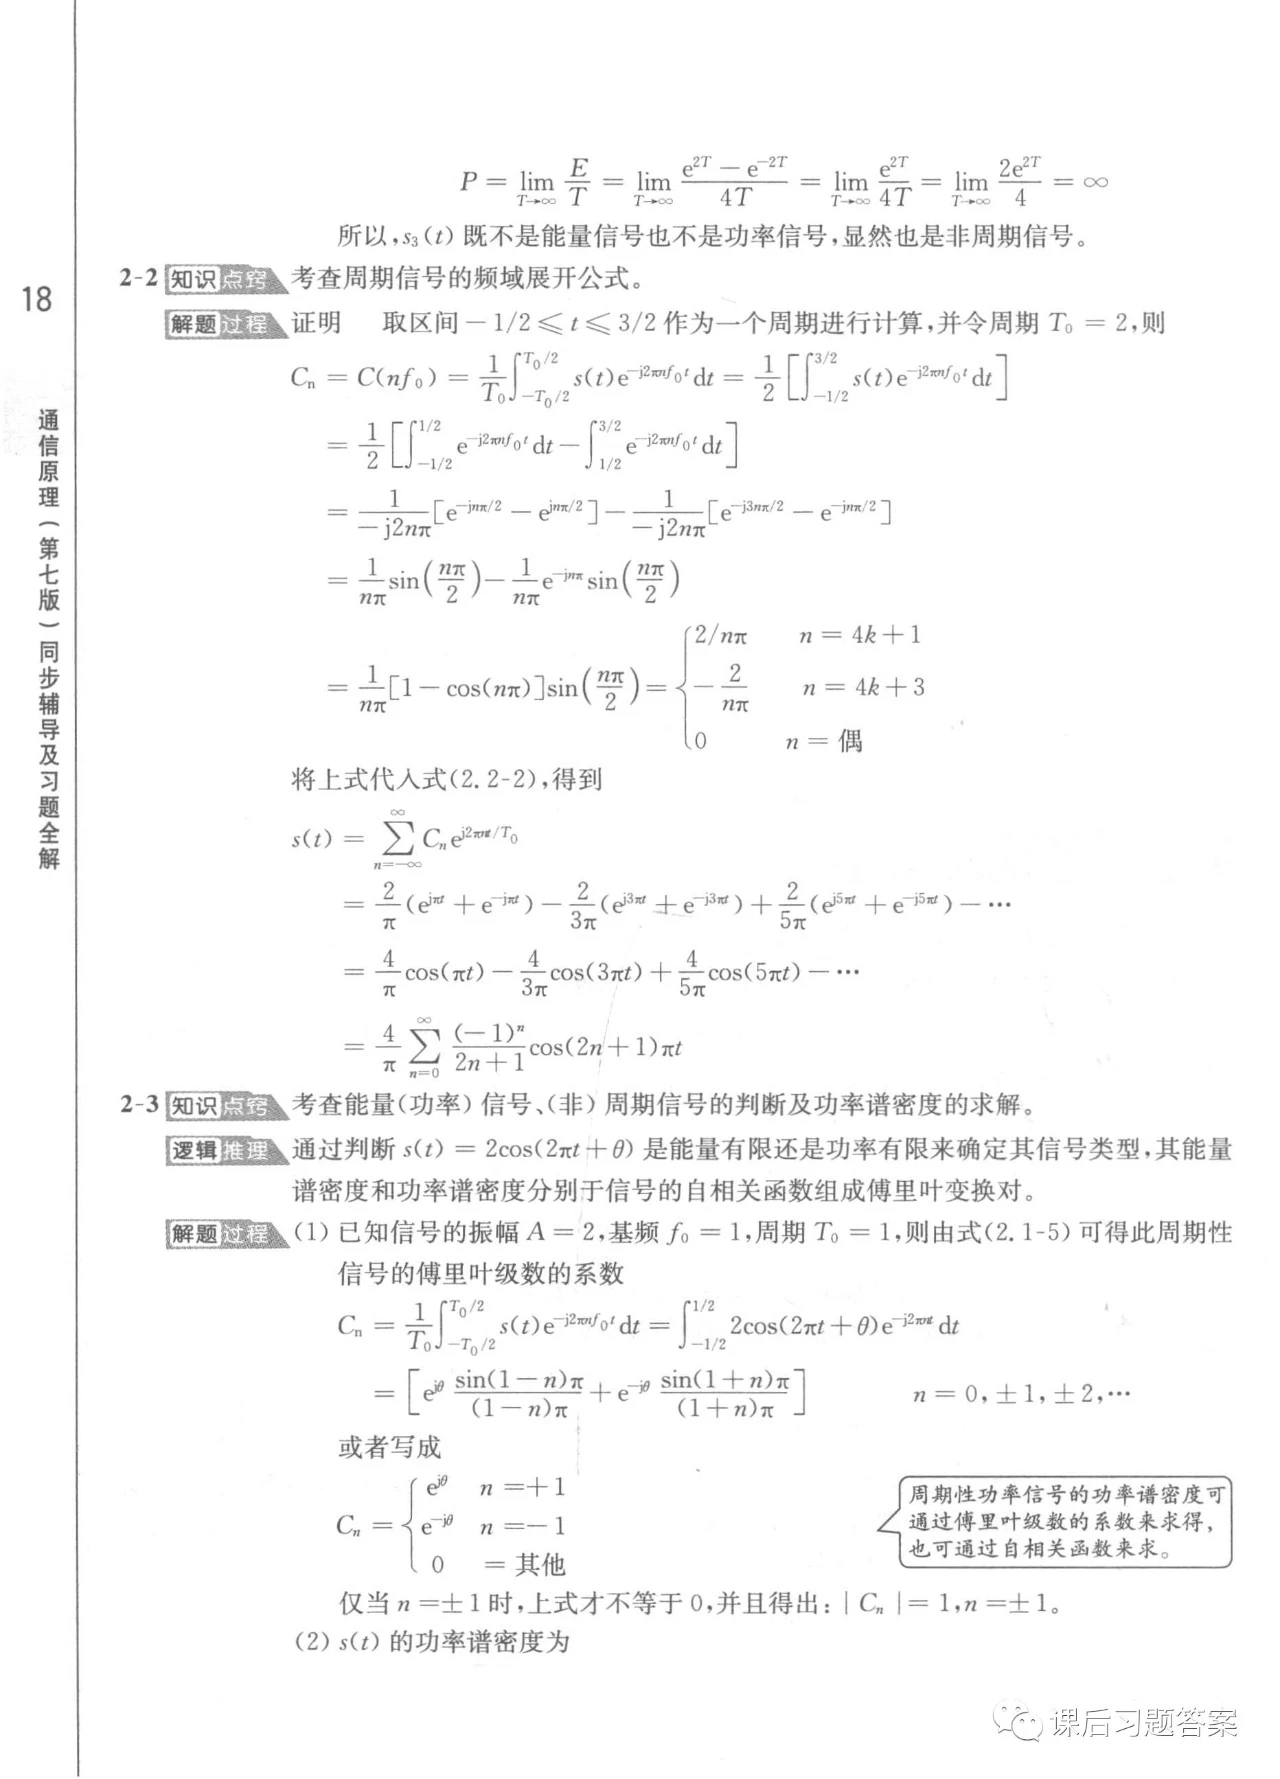
\includegraphics[height=4.0cm,width=4.5cm]{pics/3.png}%figures文件夹下的DSC.png图片,
	\caption{三阶展开电路设计}
\end{figure}
其中,电源电压的幅值以及频率均不相等,通过计算三个电源的幅值分别为:$1.27V、0.42V、0.25V$,频率分别为50Hz、150Hz、250Hz.

利用orCAD软件连接电路图,并利用Pspice对图3电路图进行仿真,仿真结果见图4.
\begin{figure}[htbp]
	\centering
	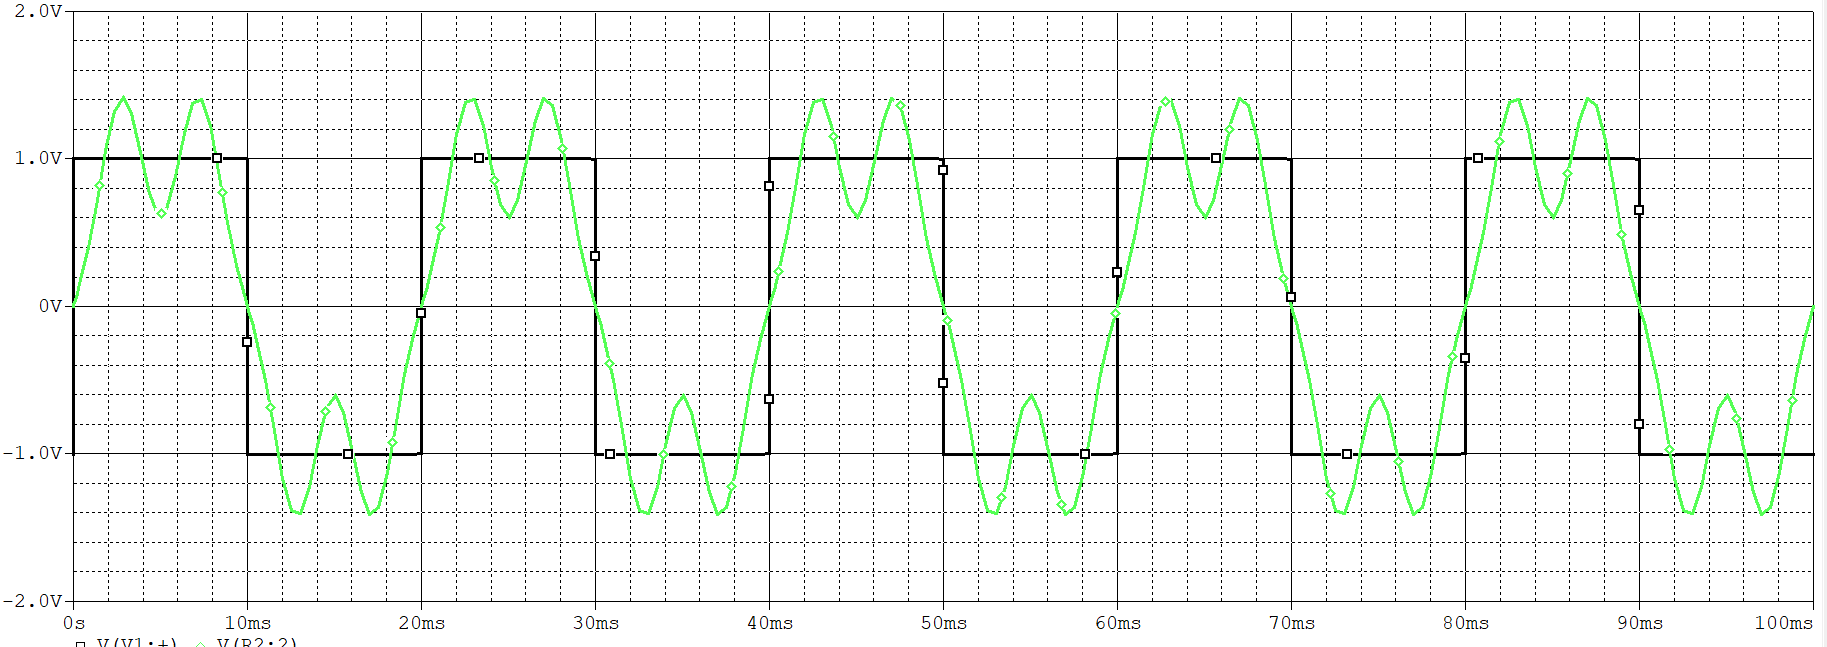
\includegraphics[height=4.0cm,width=12cm]{pics/3fangzhen.png}%figures文件夹下的DSC.png图片,
	\caption{三阶展开仿真图}
\end{figure}

其中类似曲线变化的为三个电源叠加的输出波形,方波为原始电路的输出曲线

观察三阶展开叠加的仿真图,发现虽然三个叠加电源的频率和幅值均不相等,但通过叠加后输出的波形为周期性变化的曲线,且驮载在展开前的输出方波上,周期大致相同.

\subsubsection*{3.2 七阶展开仿真}
与三阶仿真相似,将输入函数进行更高阶的展开,利用多个正弦交流源叠加,观察其输出波形的情况.为了方便起见,这里对方波信号进行七阶展开,即七个电源进行叠加.
设计电路图见图5.

\begin{figure}[htbp]
	\centering
	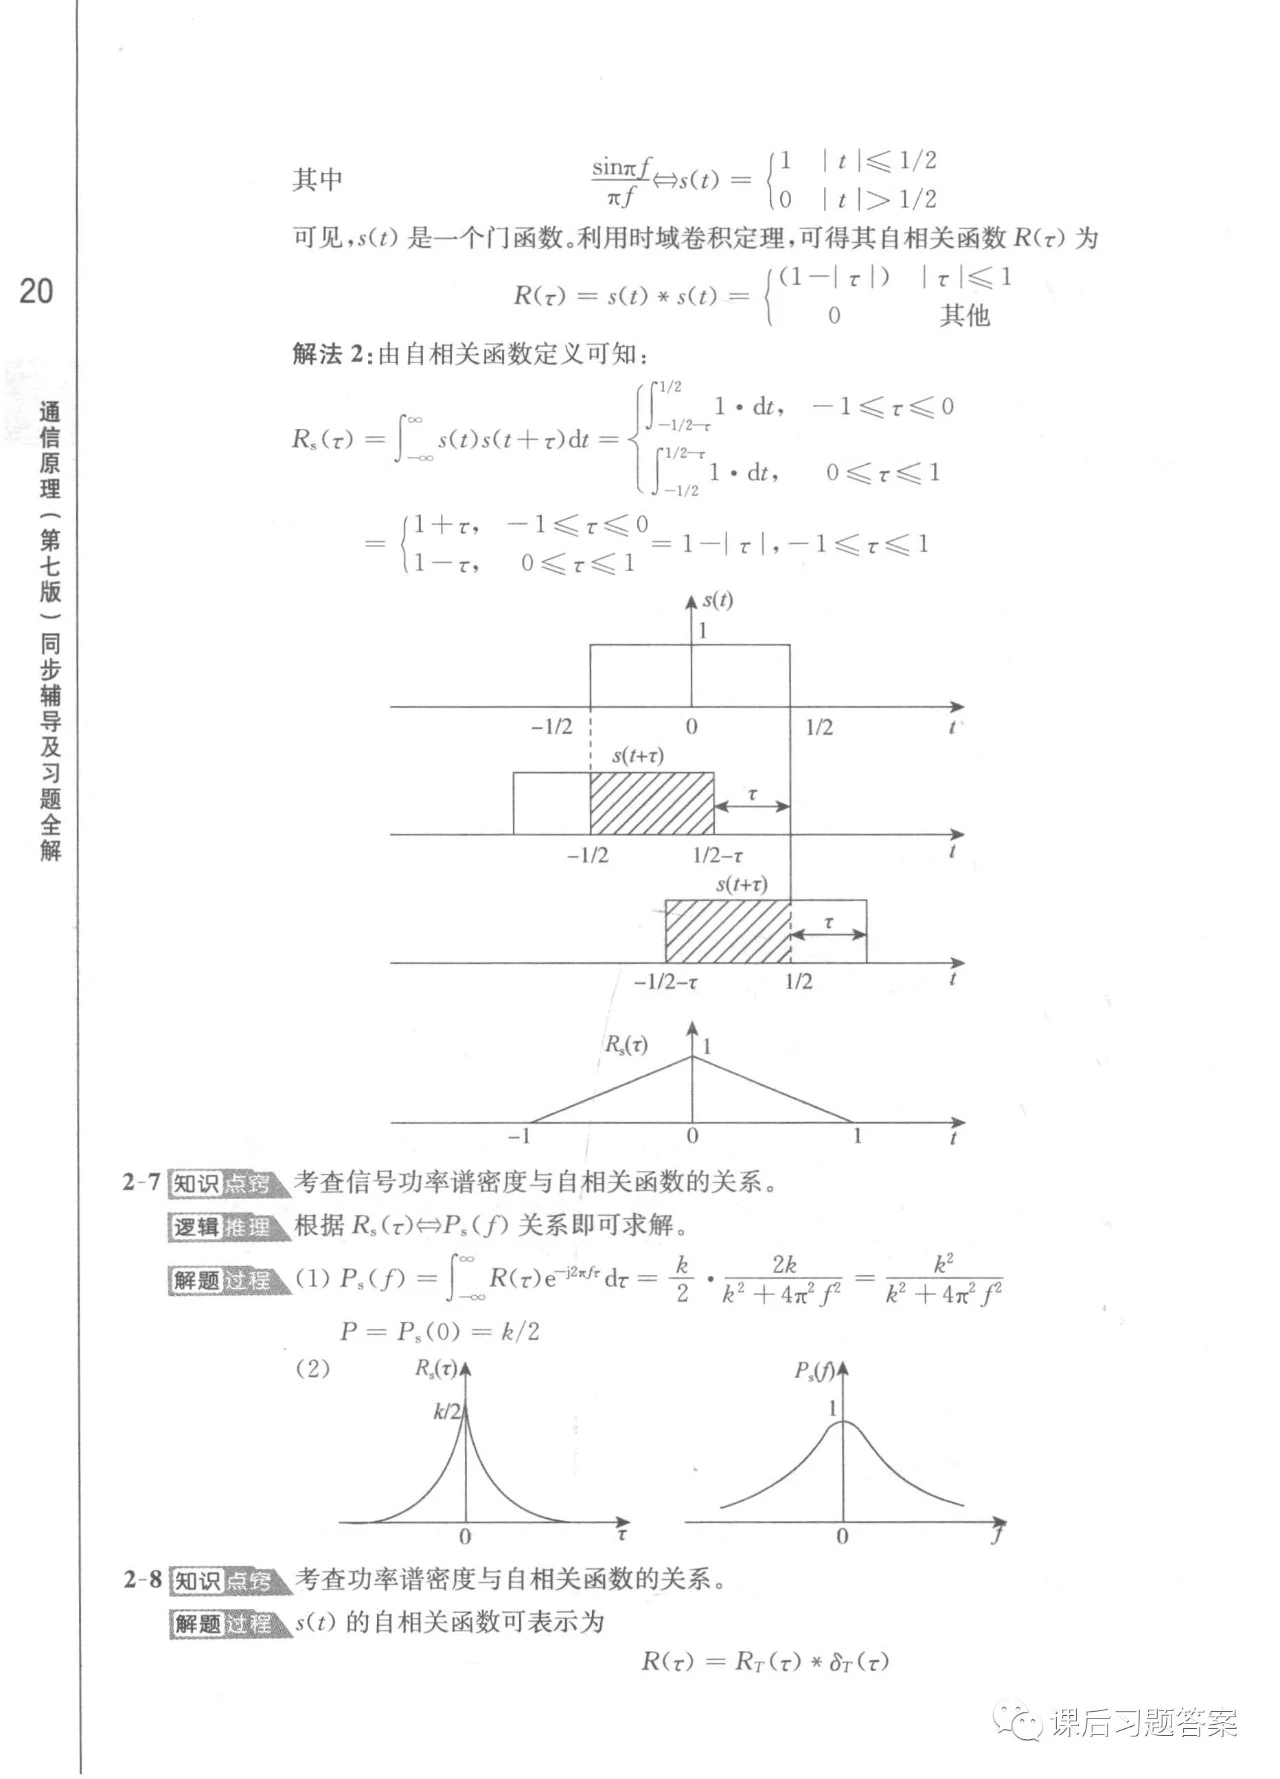
\includegraphics[height=4.0cm,width=7.5cm]{pics/5.png}%figures文件夹下的DSC.png图片,
	\caption{七阶展开电路设计}
\end{figure}

利用orCAD软件连接电路图,并利用Pspice对图5电路图进行仿真,仿真结果见图6.

\begin{figure}[htbp]
	\centering
	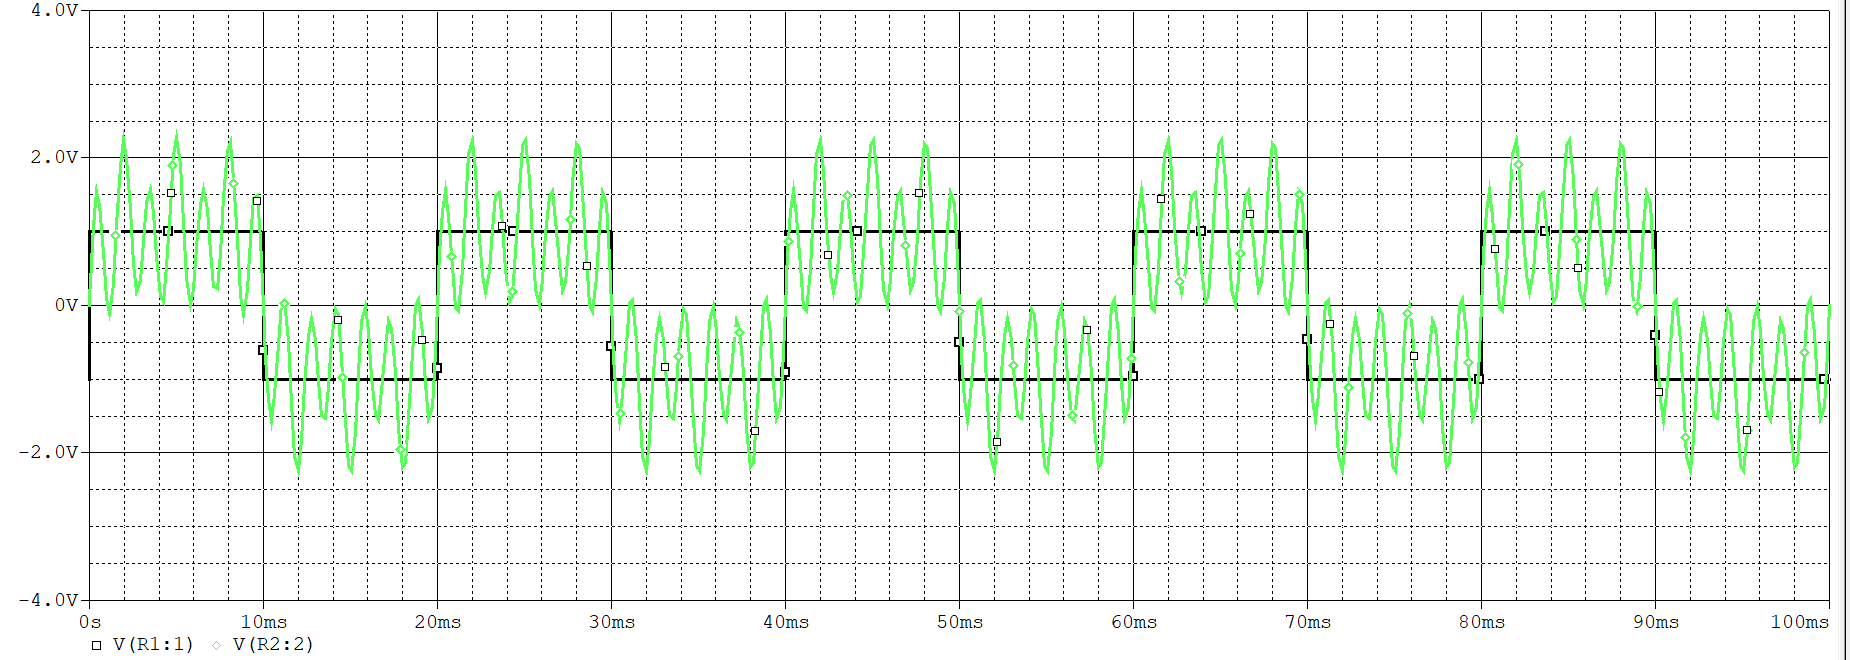
\includegraphics[height=5.0cm,width=12cm]{pics/7fangzhen.png}%figures文件夹下的DSC.png图片,
	\caption{七阶展开仿真图}
\end{figure}

输出波形驮载在未展开的方波信号上,且与方波信号更相似.

由此,可以得出结论:将方波信号进行无穷阶的傅里叶级数展开,其输出波形将无限接近方波信号.

\textbf{你眼中看似落叶纷飞变化无常的世界,实际只是躺在上帝怀中一份早已谱好的乐章.}
\end{document}
